\documentclass{article}
\usepackage[utf8]{inputenc}
\usepackage[margin=0.70in]{geometry}
\usepackage{graphicx}

\title{HW 2-3: Parallelizing Particle Simulation Using CUDA and GPU}
\author{Andrew Chen, Xuan Jiang, Brian Park}
\date{March 2022}

\begin{document}

\maketitle

\section{Code}
\subsection{Data Structures}
\begin{itemize}
    \item \verb|bin_ids| \\
        This holds the head of the pointer of the next reference of the particle in the bin in \verb|particle_ids|.
    \item \verb|particle_ids| \\
        This is a mapping and reference of the particle ids. In it is stored \verb|len(bin_ids)| linked list, where each linked list contains the particle in that specific bin. The element inside \verb|particle_ids| will point to the next index of the particle. The end of the linked list or the null pointer is encoded as -1.
    
\end{itemize}

\subsection{Algorithm}
In general, compared to using prefix sum, this saves on memory allocation, but may seem to take a hit on spatial locality, since the linked list is not stored contiguously and cannot take advantage of the GPU cache. Another tradeoff that this design has is that it does not need to sort and can append to the linked list in $O(1)$ time using an atomic swap primitive in CUDA. Thus, the creation of the linked list can be called by a \verb|__global__| function, although the actual appending takes $O(n)$ time for each iteration per bin. But note that as the number of particles increase, the more bins that are created, so each bin will have a relatively small amount of particles, thus the $O(n)$ time mentioned earlier is smaller and latency of pointer chasing is essentially hidden to a smaller constant as you increase the number of particles. 

\subsection{Synchronization}
The only synchronization primitive that this code uses are atomic instructions \verb|atomicExch()|, \verb|atomicAdd()| and \\ \verb|__syncthreads()|. We need \verb|atomicExch()| to append the linked list atomically and update the head of the head of the \verb|bin_ids| table of references. We need \verb|__syncthreads()| during the end of \verb|compute_forces_gpu_bin()| because we rebin the particles every time after moving. This is a GPU kernel level synchronization that should ensure this correctness. Otherwise, the code may decide to bin particles without finishing moving. We also had to change the starter code and include \verb|atomicAdd()| in \verb|apply_force_gpu()|. In order to algorithmically speed up our code by including bidirectional iteration, we needed to add atomics as GPU threads would often collide and give incorrect results when updating particle metadata. 

\subsection{Other Design Choices}
Originally, we tried to use the GSI's recitation slides as a guide, using the prefix sum to compute the location of the \verb|particle_ids| into \verb|bin_ids| as the pointer to the location, since \verb|particles| would be sorted and stored contiguously into \verb|particle_ids|. But we had a lot of trouble figuring out how to make this ensure correctness, as in \verb|init_simulation| everything would seem correct, but after iterations in \verb|simulate_one_step|  there was synchronization issues where sometimes the bins wouldn't be sorted properly. Adding synchronization primitives such as \verb|cudaDeviceSynchronize()| and \verb|__syncthreads()| only slowed down the code and didn't fix correctness. Due to this weird correctness bug, we started from scratch again. We had the linked list implementation in mind, but were worried that pointer chasing would incur a lot of GPU cache misses. Given that the GPU architecture is very expensive and performant on registers and memory bandwidth, this type of concern should be free and very minimal. The linked list implementation is under 4 seconds and pretty good compared to previous semester grades, we merged it into our main implementation. Ignoring correctness, the performance of prefix sum and sorting implementation was very bad, and it was probably due to the calls of \verb|cudaMemCpy| to do transfer data from CPU to GPU. Fortunately, the linked list implementation resides all of its computation on the GPU memory. Surprisingly, the code is very straightforward and cleaner than the original prefix sum and sorting implementation.

\subsection{Can We Do Better?}
If given enough time, abandoning the linked list implementation and redoing the prefix sum could give us better performance. But considering that a student on Piazza reached 1.5 seconds on 1 million particles (ours is around 1.26s), we considered this as our stopping point. To implement the prefix sum required more code and a lot more debugging, and it was frustrating to use \verb|cuda-gdb| as switching into GPU kernel threads was often confusing to understand. Instead, we printed statements by transferring copies to CPU for correctness.

\section{Performance}

\subsection{Log-Log Plot of Naive and GPU Implementation with Linear Behavior}
\centerline{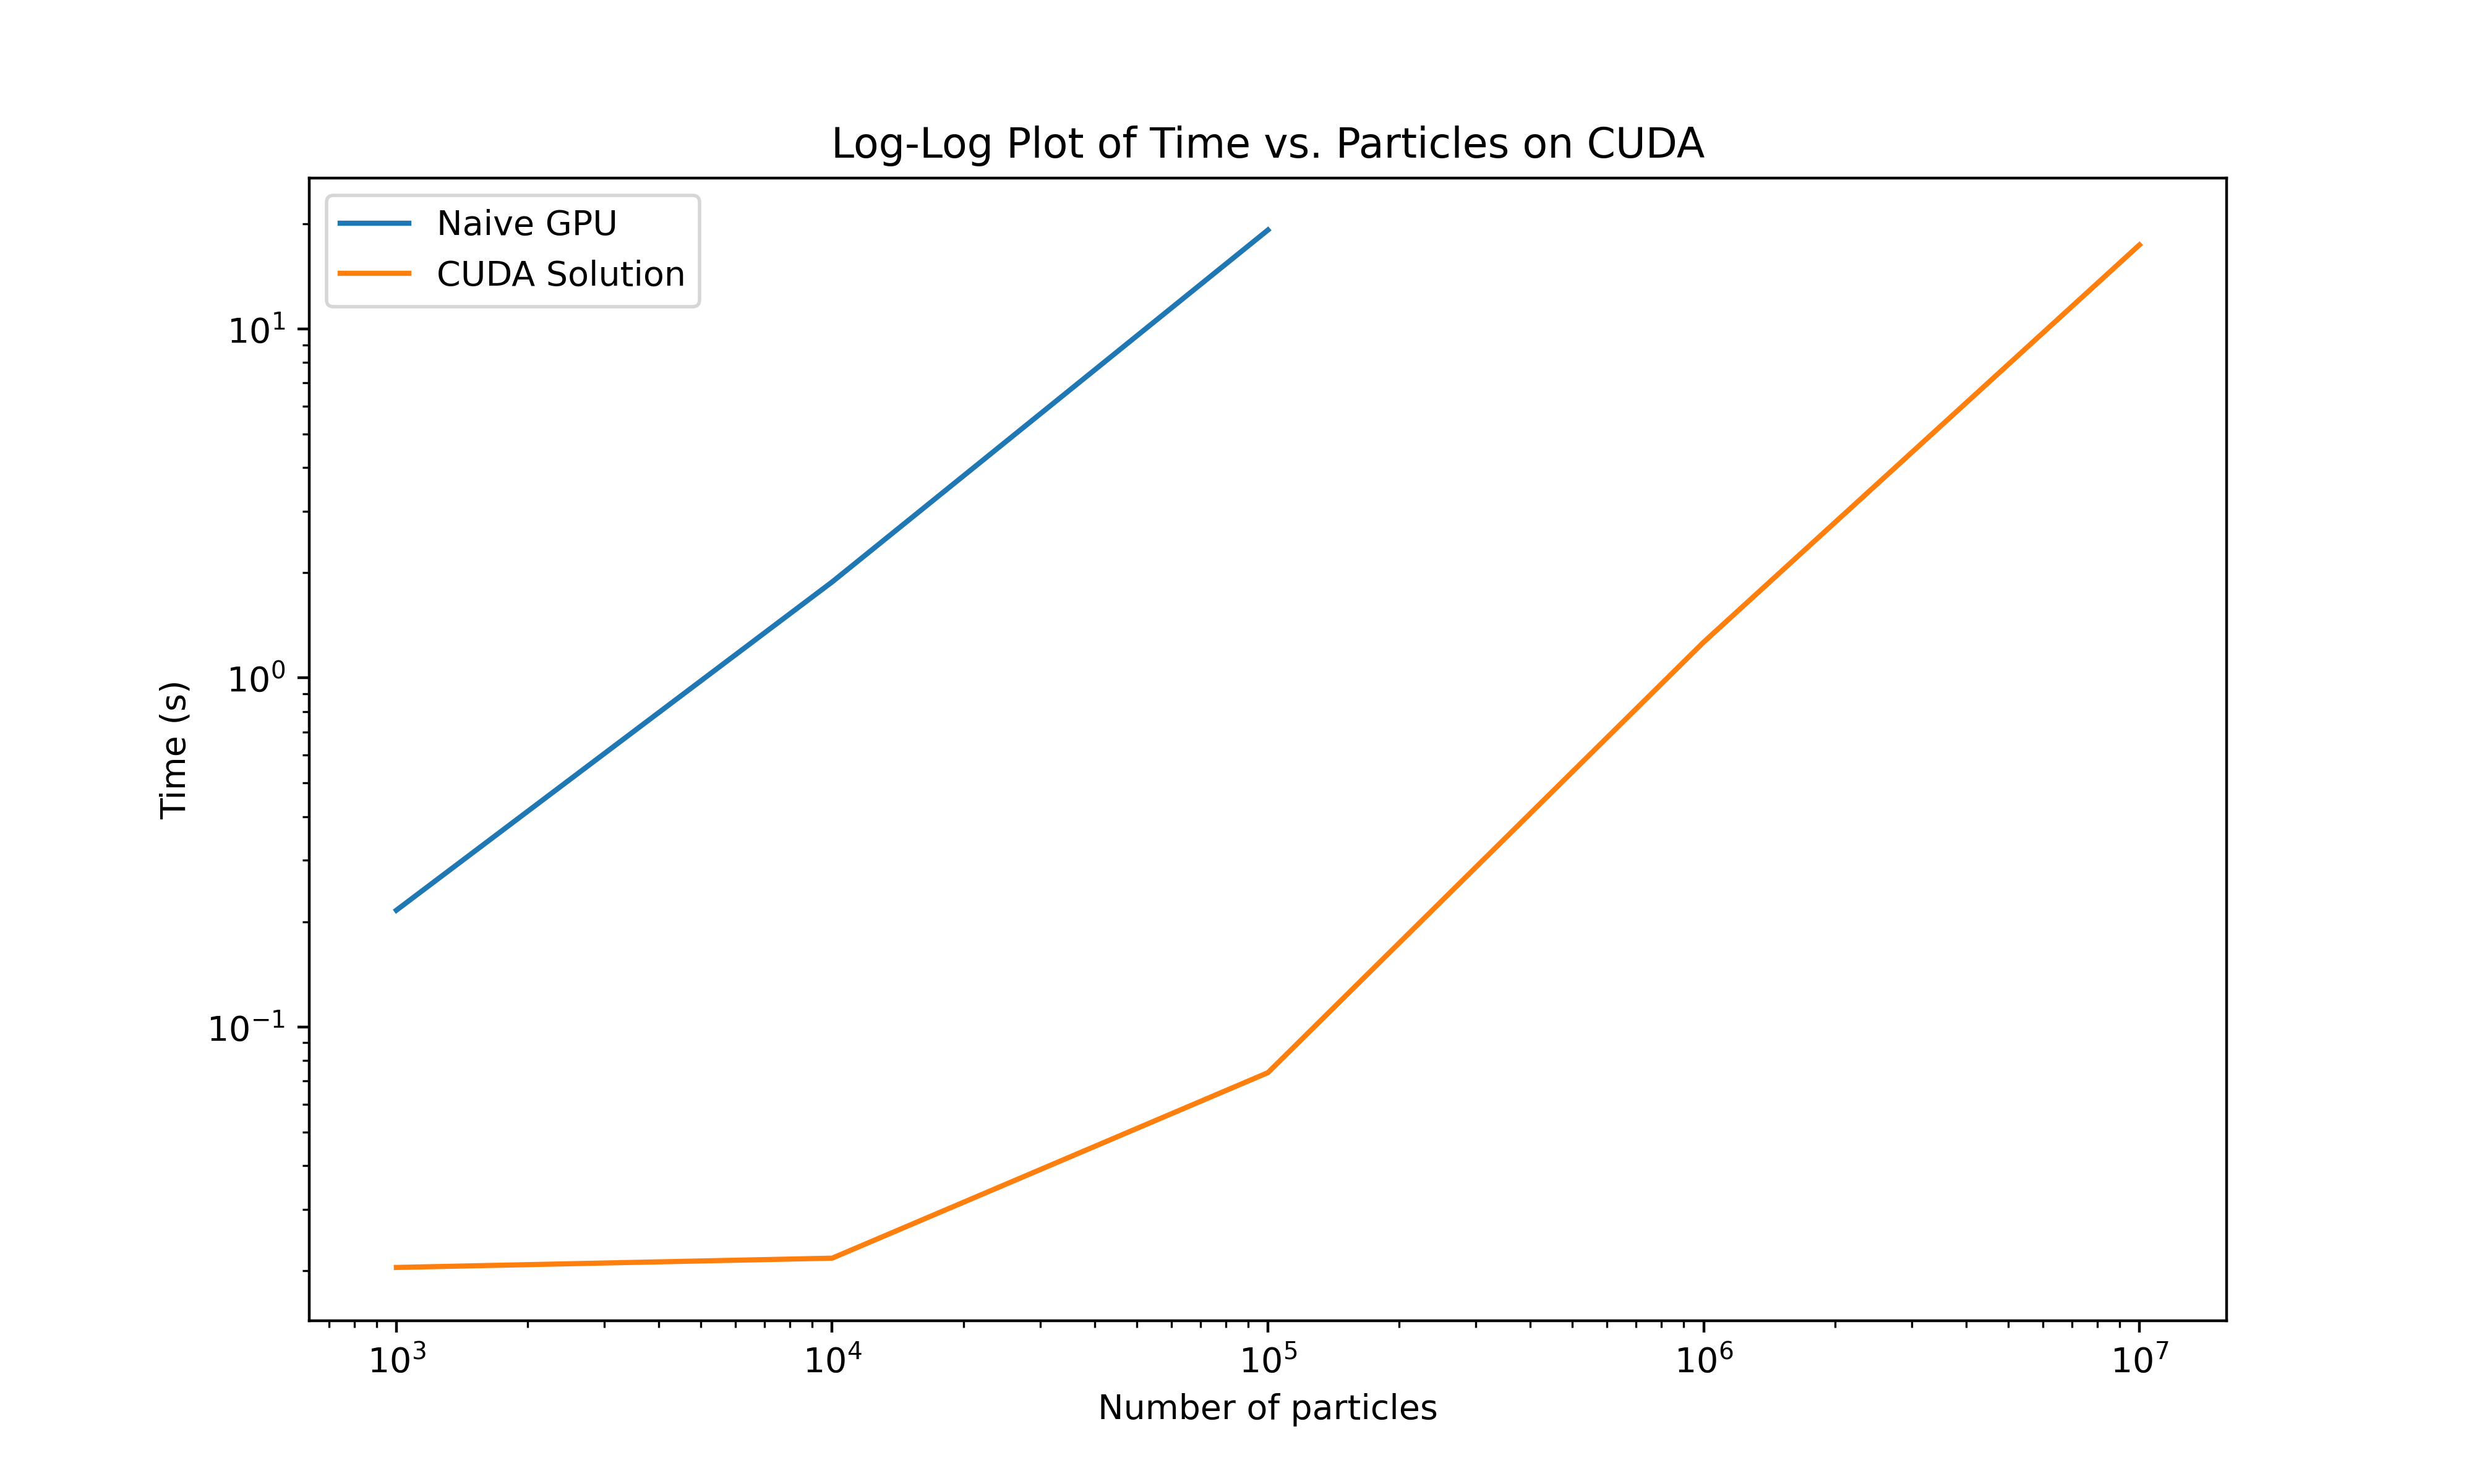
\includegraphics[width=6in]{figures/log-log.png}}

Above shows the plots of the GPU optimized performance compared to the naive implementation from the starter code. We have a constant increase in performance for naive and our optimized solution is able to follow that increase but at a much lower time. This is essentially the Roofline model in effect, where we see our performance be in memory bound and change to compute bound at around $10^5$ particles.


\subsection{All Implmentations of HW 2 Compared}
\centerline{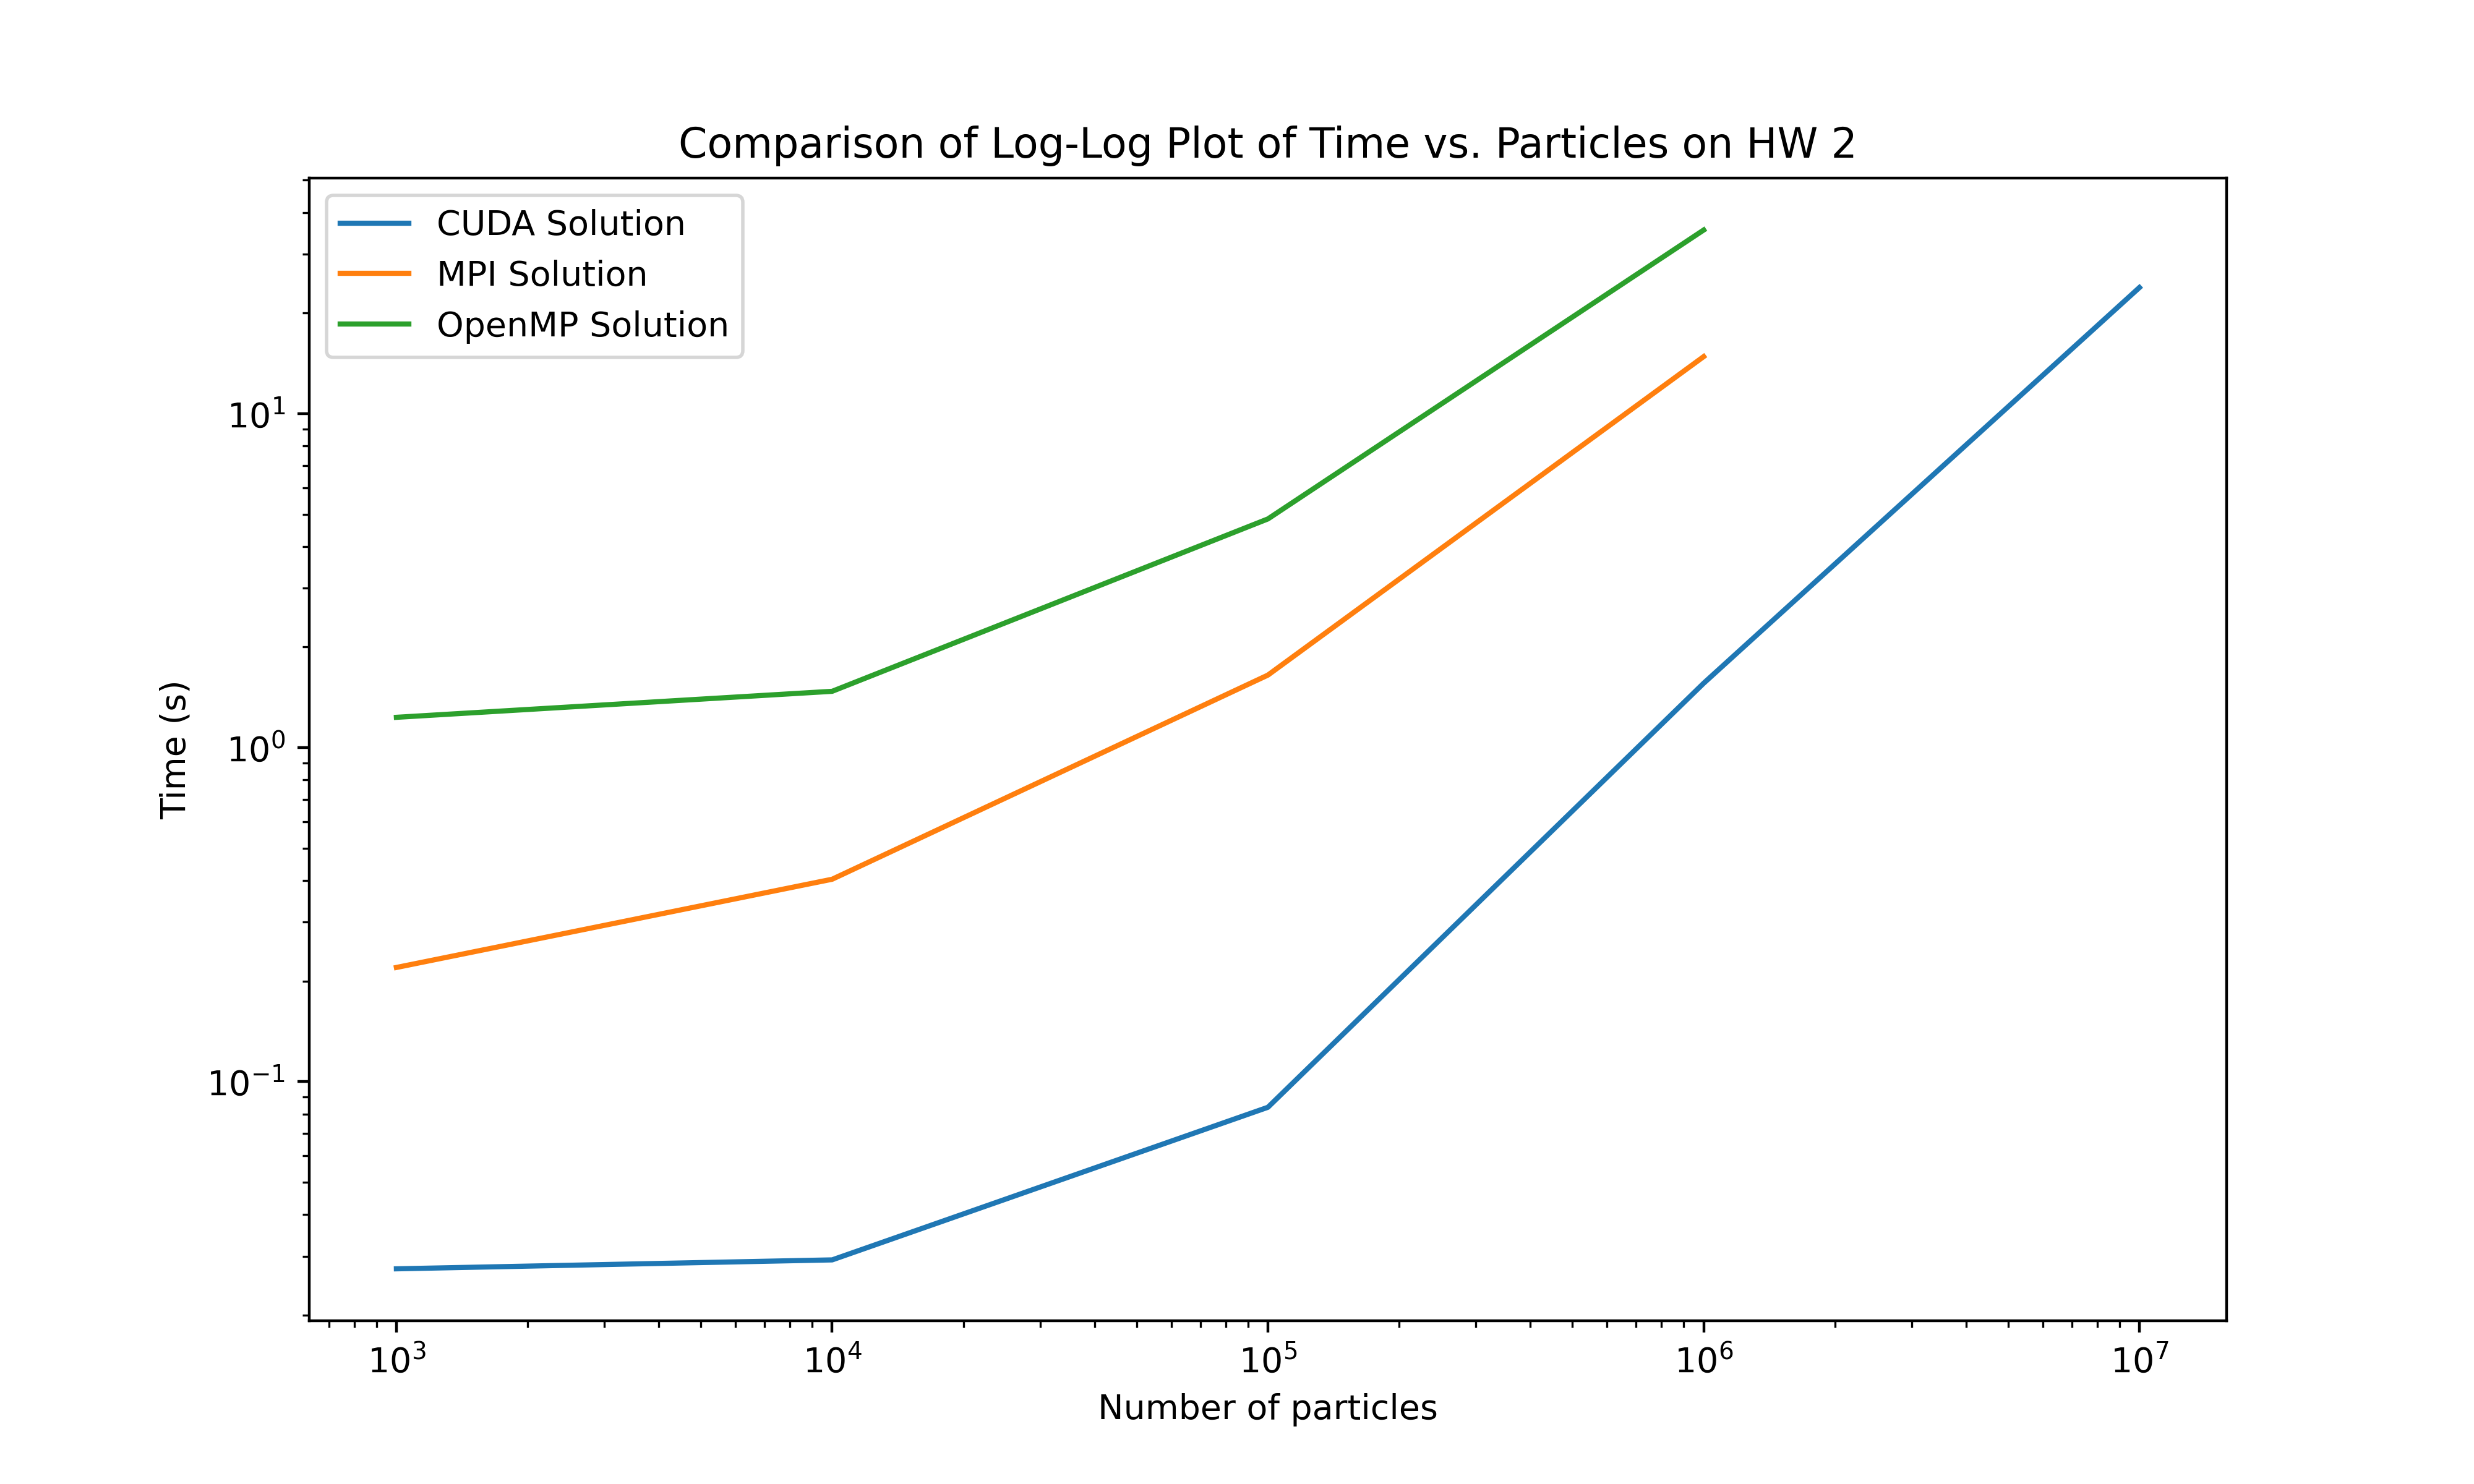
\includegraphics[width=6in]{figures/hw2-compare.png}}

Interestingly, we see all of our implementations from OpenMP, MPI, and CUDA graphed together. Amazingly, CUDA beats all of the implementation time wise. While benchmarking, we could not test 10 million particles on OpenMP and MPI as it would take too long. But even at 1 million particles, it's amazing to see how adding hardware improves speed by a lot. Notes that OpenMP was run on 68 threads on Cori, and MPI was run on 2 nodes with 68 processes (total 136 processes). Both were on Cori KNL nodes while CUDA was on bridges-2 node with 1 Nvidia Tesla V100 GPU (a whopping 5120 CUDA cores).

\subsection{Profiling}
Here is a dump of the profiling log from \verb|nvprof| for 1000 particles:

\begin{verbatim}
 GPU activities:   63.15%  7.8961ms      1000  7.8960us  3.8400us  9.3760us  compute_forces_gpu_bin
                                                                (particle_t*, int, int, double, int*, int*)
                   20.81%  2.6014ms      1000  2.6010us  2.5590us  2.8480us  move_gpu
                                                                (particle_t*, int, double)
                   15.99%  1.9989ms      1001  1.9960us  1.9190us  2.6880us  binning
                                                                (particle_t*, int, int, double, int*, int*)
                    0.05%  6.7520us         1  6.7520us  6.7520us  6.7520us  [CUDA memcpy HtoD]
      API calls:   90.32%  213.51ms         3  71.170ms  3.2540us  213.50ms  cudaMalloc
                    4.72%  11.163ms      3001  3.7190us  3.2580us  32.592us  cudaLaunchKernel
                    4.37%  10.341ms      1001  10.330us  1.1000us  18.366us  cudaDeviceSynchronize
                    0.27%  632.12us         1  632.12us  632.12us  632.12us  cuDeviceTotalMem
                    0.25%  592.64us       101  5.8670us     124ns  264.68us  cuDeviceGetAttribute
                    0.04%  87.428us         1  87.428us  87.428us  87.428us  cuDeviceGetName
                    0.02%  39.854us         1  39.854us  39.854us  39.854us  cudaMemcpy
                    0.00%  10.101us         1  10.101us  10.101us  10.101us  cudaFree
                    0.00%  9.7660us         1  9.7660us  9.7660us  9.7660us  cuDeviceGetPCIBusId
                    0.00%  1.3440us         2     672ns     144ns  1.2000us  cuDeviceGet
                    0.00%     992ns         3     330ns     174ns     634ns  cuDeviceGetCount
                    0.00%     237ns         1     237ns     237ns     237ns  cuDeviceGetUuid
\end{verbatim}

Unless profiling creates some overhead, we know that in general, it takes around 0.020 seconds or 20ms for 1000 particles. We see that 63\% of the GPU's time is spent on \verb|compute_forces_gpu|, which is obviously the bottleneck even on serial implementation. Surprisingly, not that much time is spend on \verb|move_gpu|, but the analysis is understandable as it doesn't do anything computationally expensive. And impressively, 
\verb|binning| takes 15\% of the GPU's time. It seems very fast to append to the linked list, and it's satisfying to know that pointer chasing doesn't seem to induce that much overhead or slowdown in performance given how binning works.

For fun, a dump of 1 million particles is shown below:

\begin{verbatim}
                Type  Time(%)      Time     Calls       Avg       Min       Max  Name
 GPU activities:   53.99%  688.40ms      1000  688.40us  641.85us  844.57us  compute_forces_gpu_bin
                                                            (particle_t*, int, int, double, int*, int*)
                   33.89%  432.18ms      1001  431.75us  398.94us  484.45us  binning
                                                            (particle_t*, int, int, double, int*, int*)
                   11.29%  143.91ms      1000  143.91us  137.92us  150.30us  move_gpu
                                                            (particle_t*, int, double)
                    0.83%  10.630ms         1  10.630ms  10.630ms  10.630ms  [CUDA memcpy HtoD]
      API calls:   82.36%  1.26246s      1001  1.2612ms  1.3870us  1.6215ms  cudaDeviceSynchronize
                   15.87%  243.32ms         3  81.105ms  236.70us  242.57ms  cudaMalloc
                    0.94%  14.429ms      3001  4.8070us  3.2350us  60.706us  cudaLaunchKernel
                    0.71%  10.834ms         1  10.834ms  10.834ms  10.834ms  cudaMemcpy
                    0.04%  632.14us         1  632.14us  632.14us  632.14us  cuDeviceTotalMem
                    0.04%  578.40us       101  5.7260us     126ns  259.78us  cuDeviceGetAttribute
                    0.03%  484.55us         1  484.55us  484.55us  484.55us  cudaFree
                    0.01%  102.29us         1  102.29us  102.29us  102.29us  cuDeviceGetName
                    0.00%  5.8710us         1  5.8710us  5.8710us  5.8710us  cuDeviceGetPCIBusId
                    0.00%  1.5100us         3     503ns     167ns  1.1120us  cuDeviceGetCount
                    0.00%     807ns         2     403ns     144ns     663ns  cuDeviceGet
                    0.00%     377ns         1     377ns     377ns     377ns  cuDeviceGetUuid
\end{verbatim}

Again, we see that with profiling, the scaling of particles scales well with the simulation. There are small shifts in percentages, such as binning and computing forces, but that is probably mainly due to the ratio between particles and bins and the number of times it can map to GPU kernels threads. At some point, binning takes more execution time then move for a certain number of particles. 

Here are more visuals to depict the profiling of GPU execution: \\

\centerline{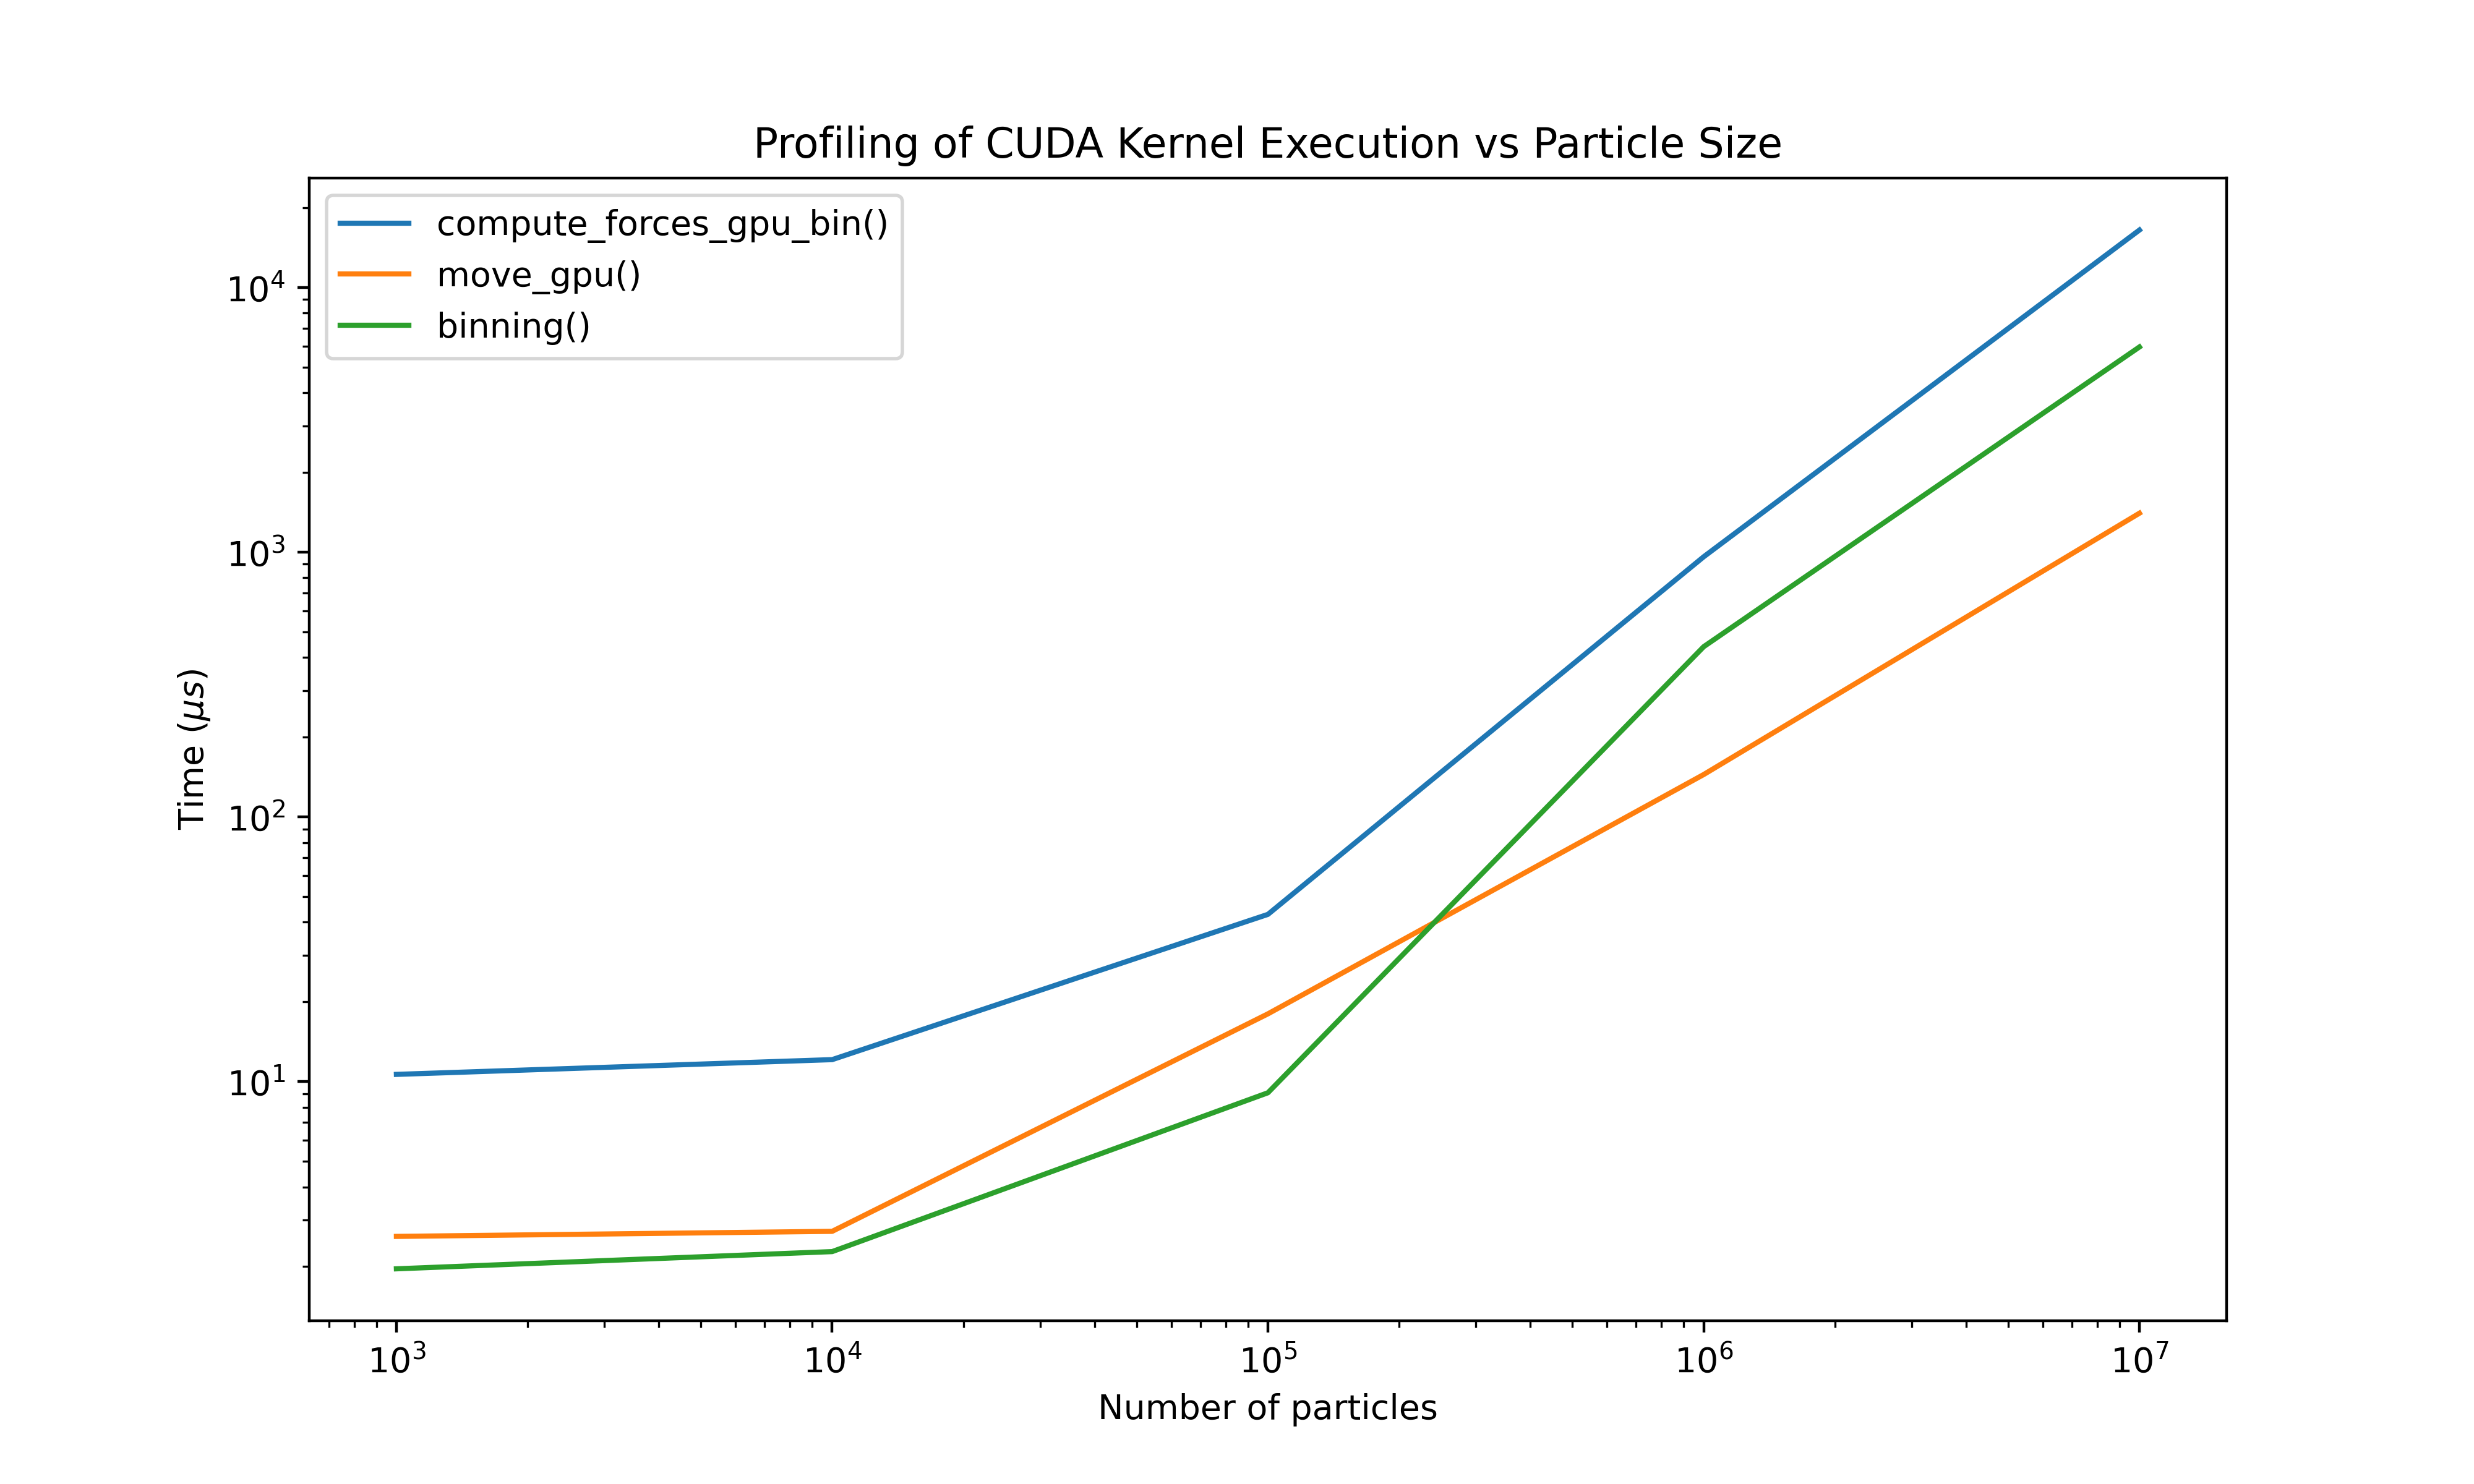
\includegraphics[width=6in]{figures/profiling.png}}

\centerline{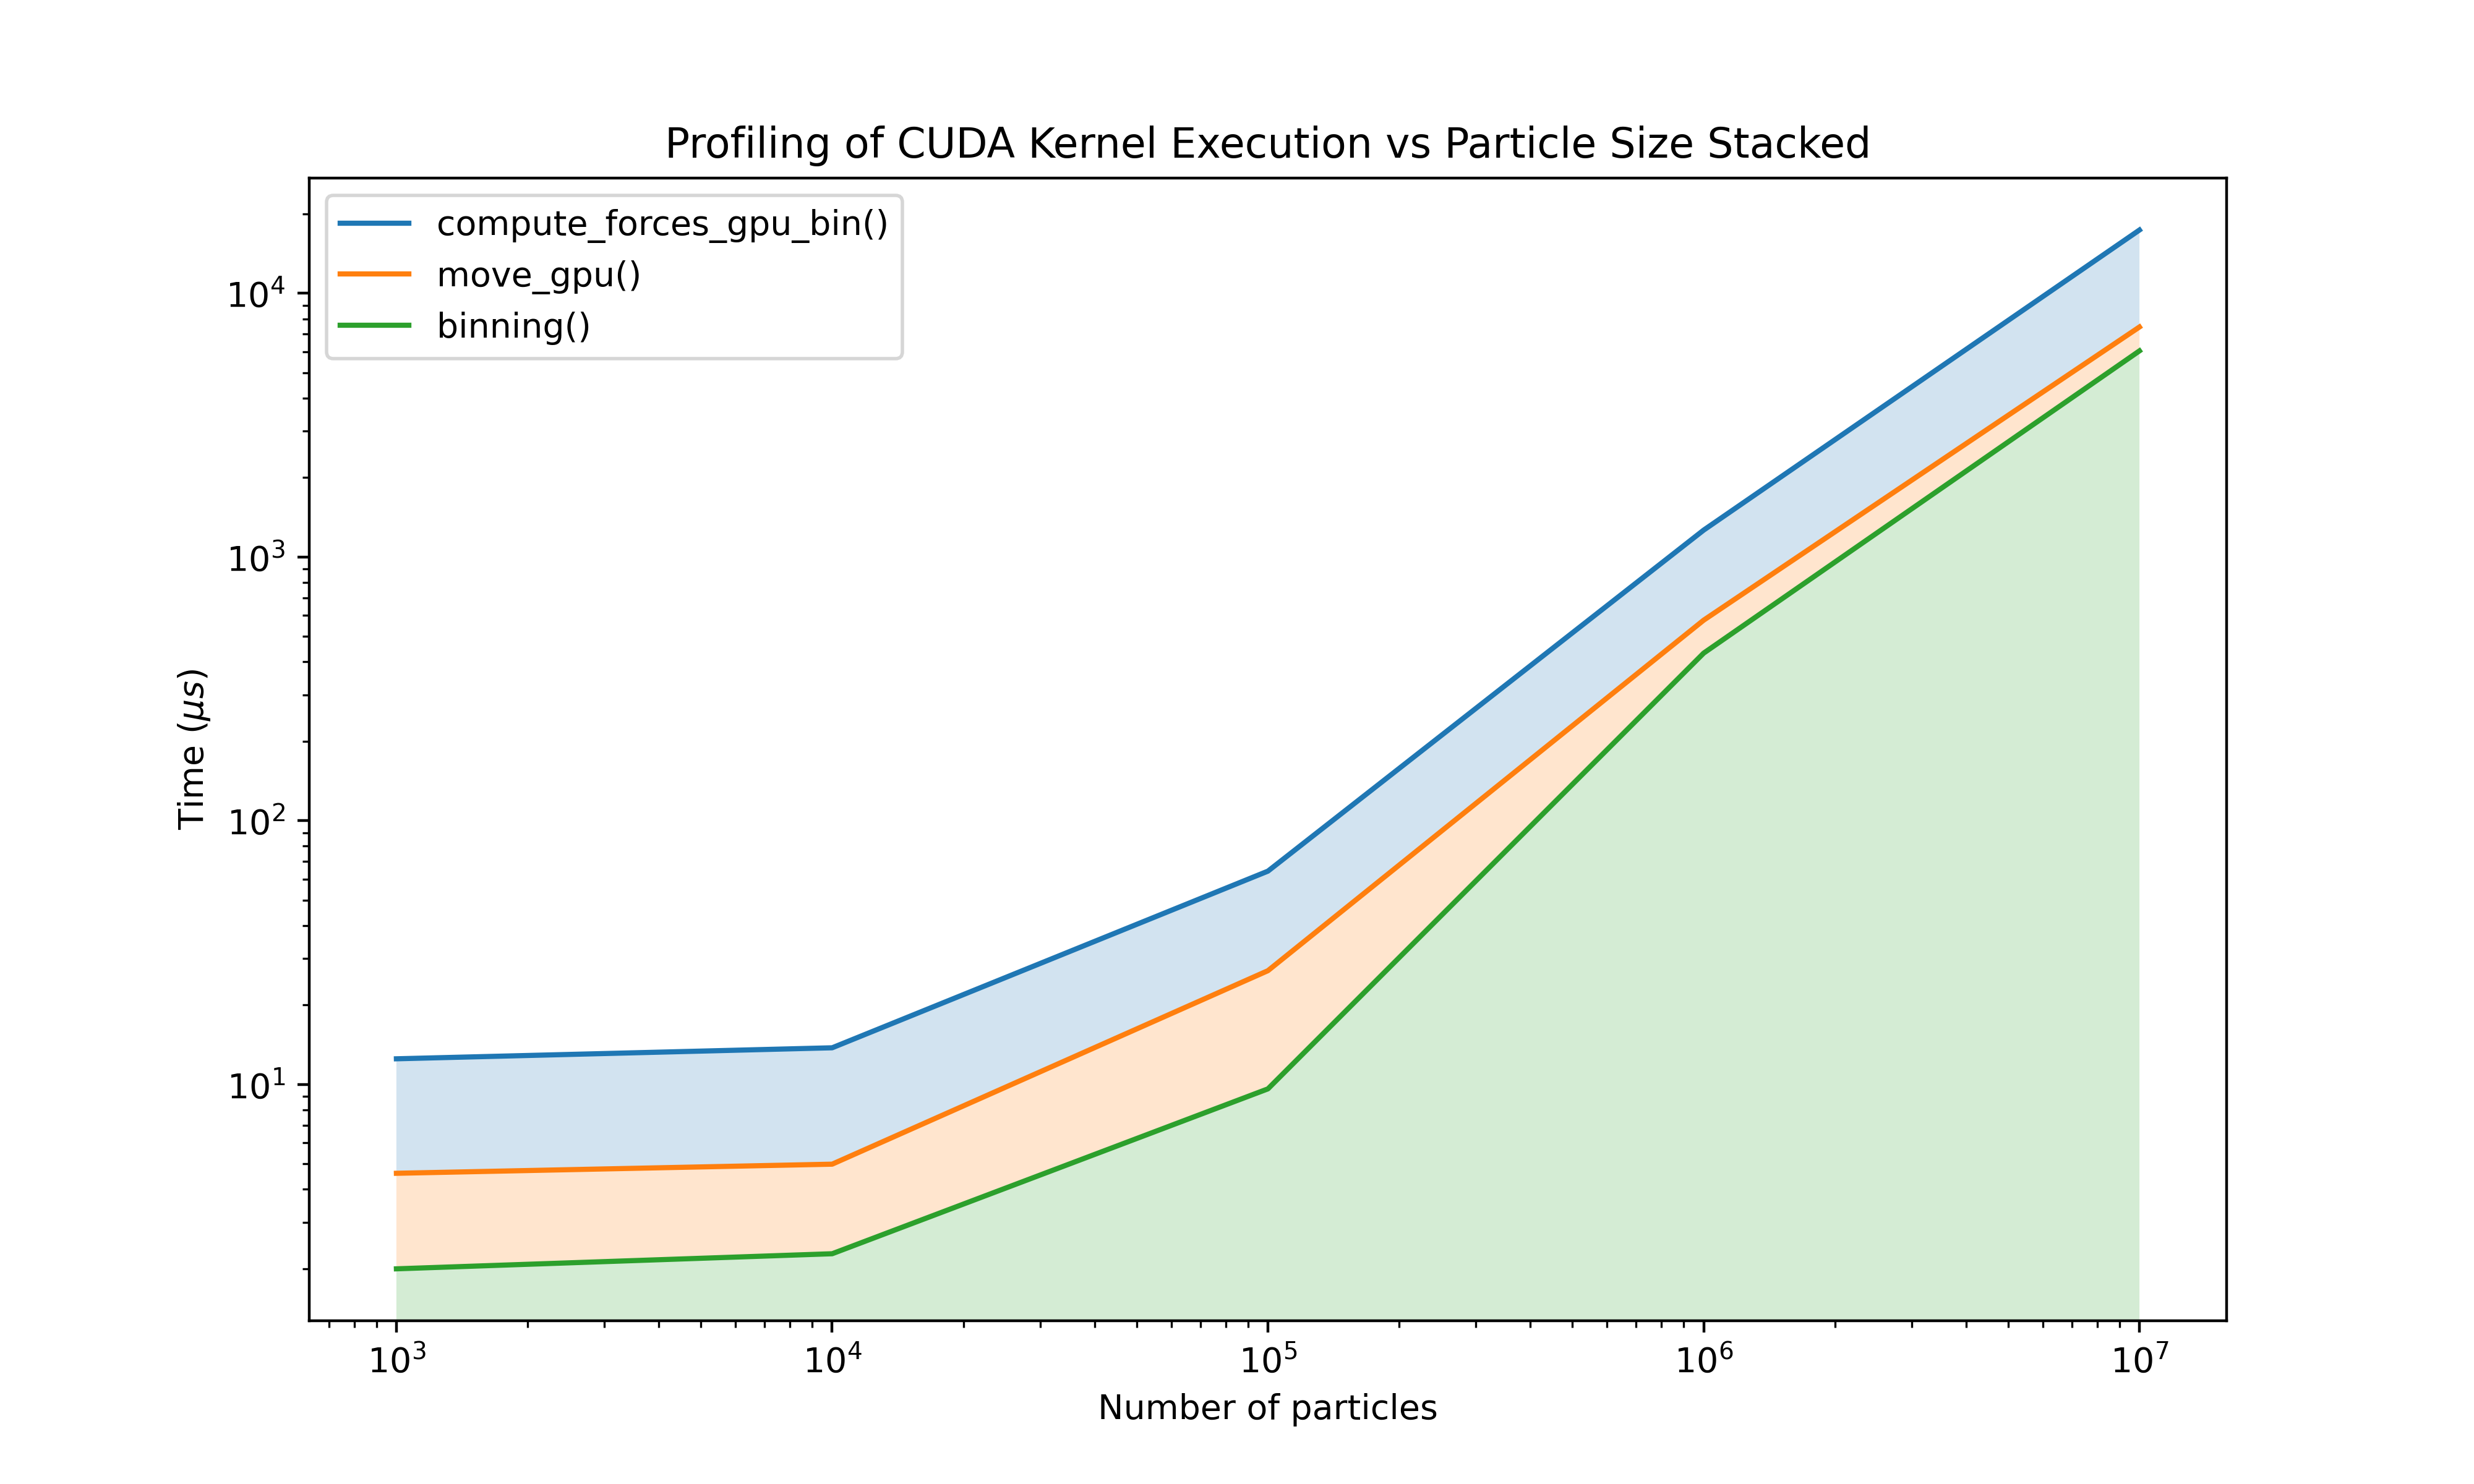
\includegraphics[width=6in]{figures/profiling-stacked.png}}

\centerline{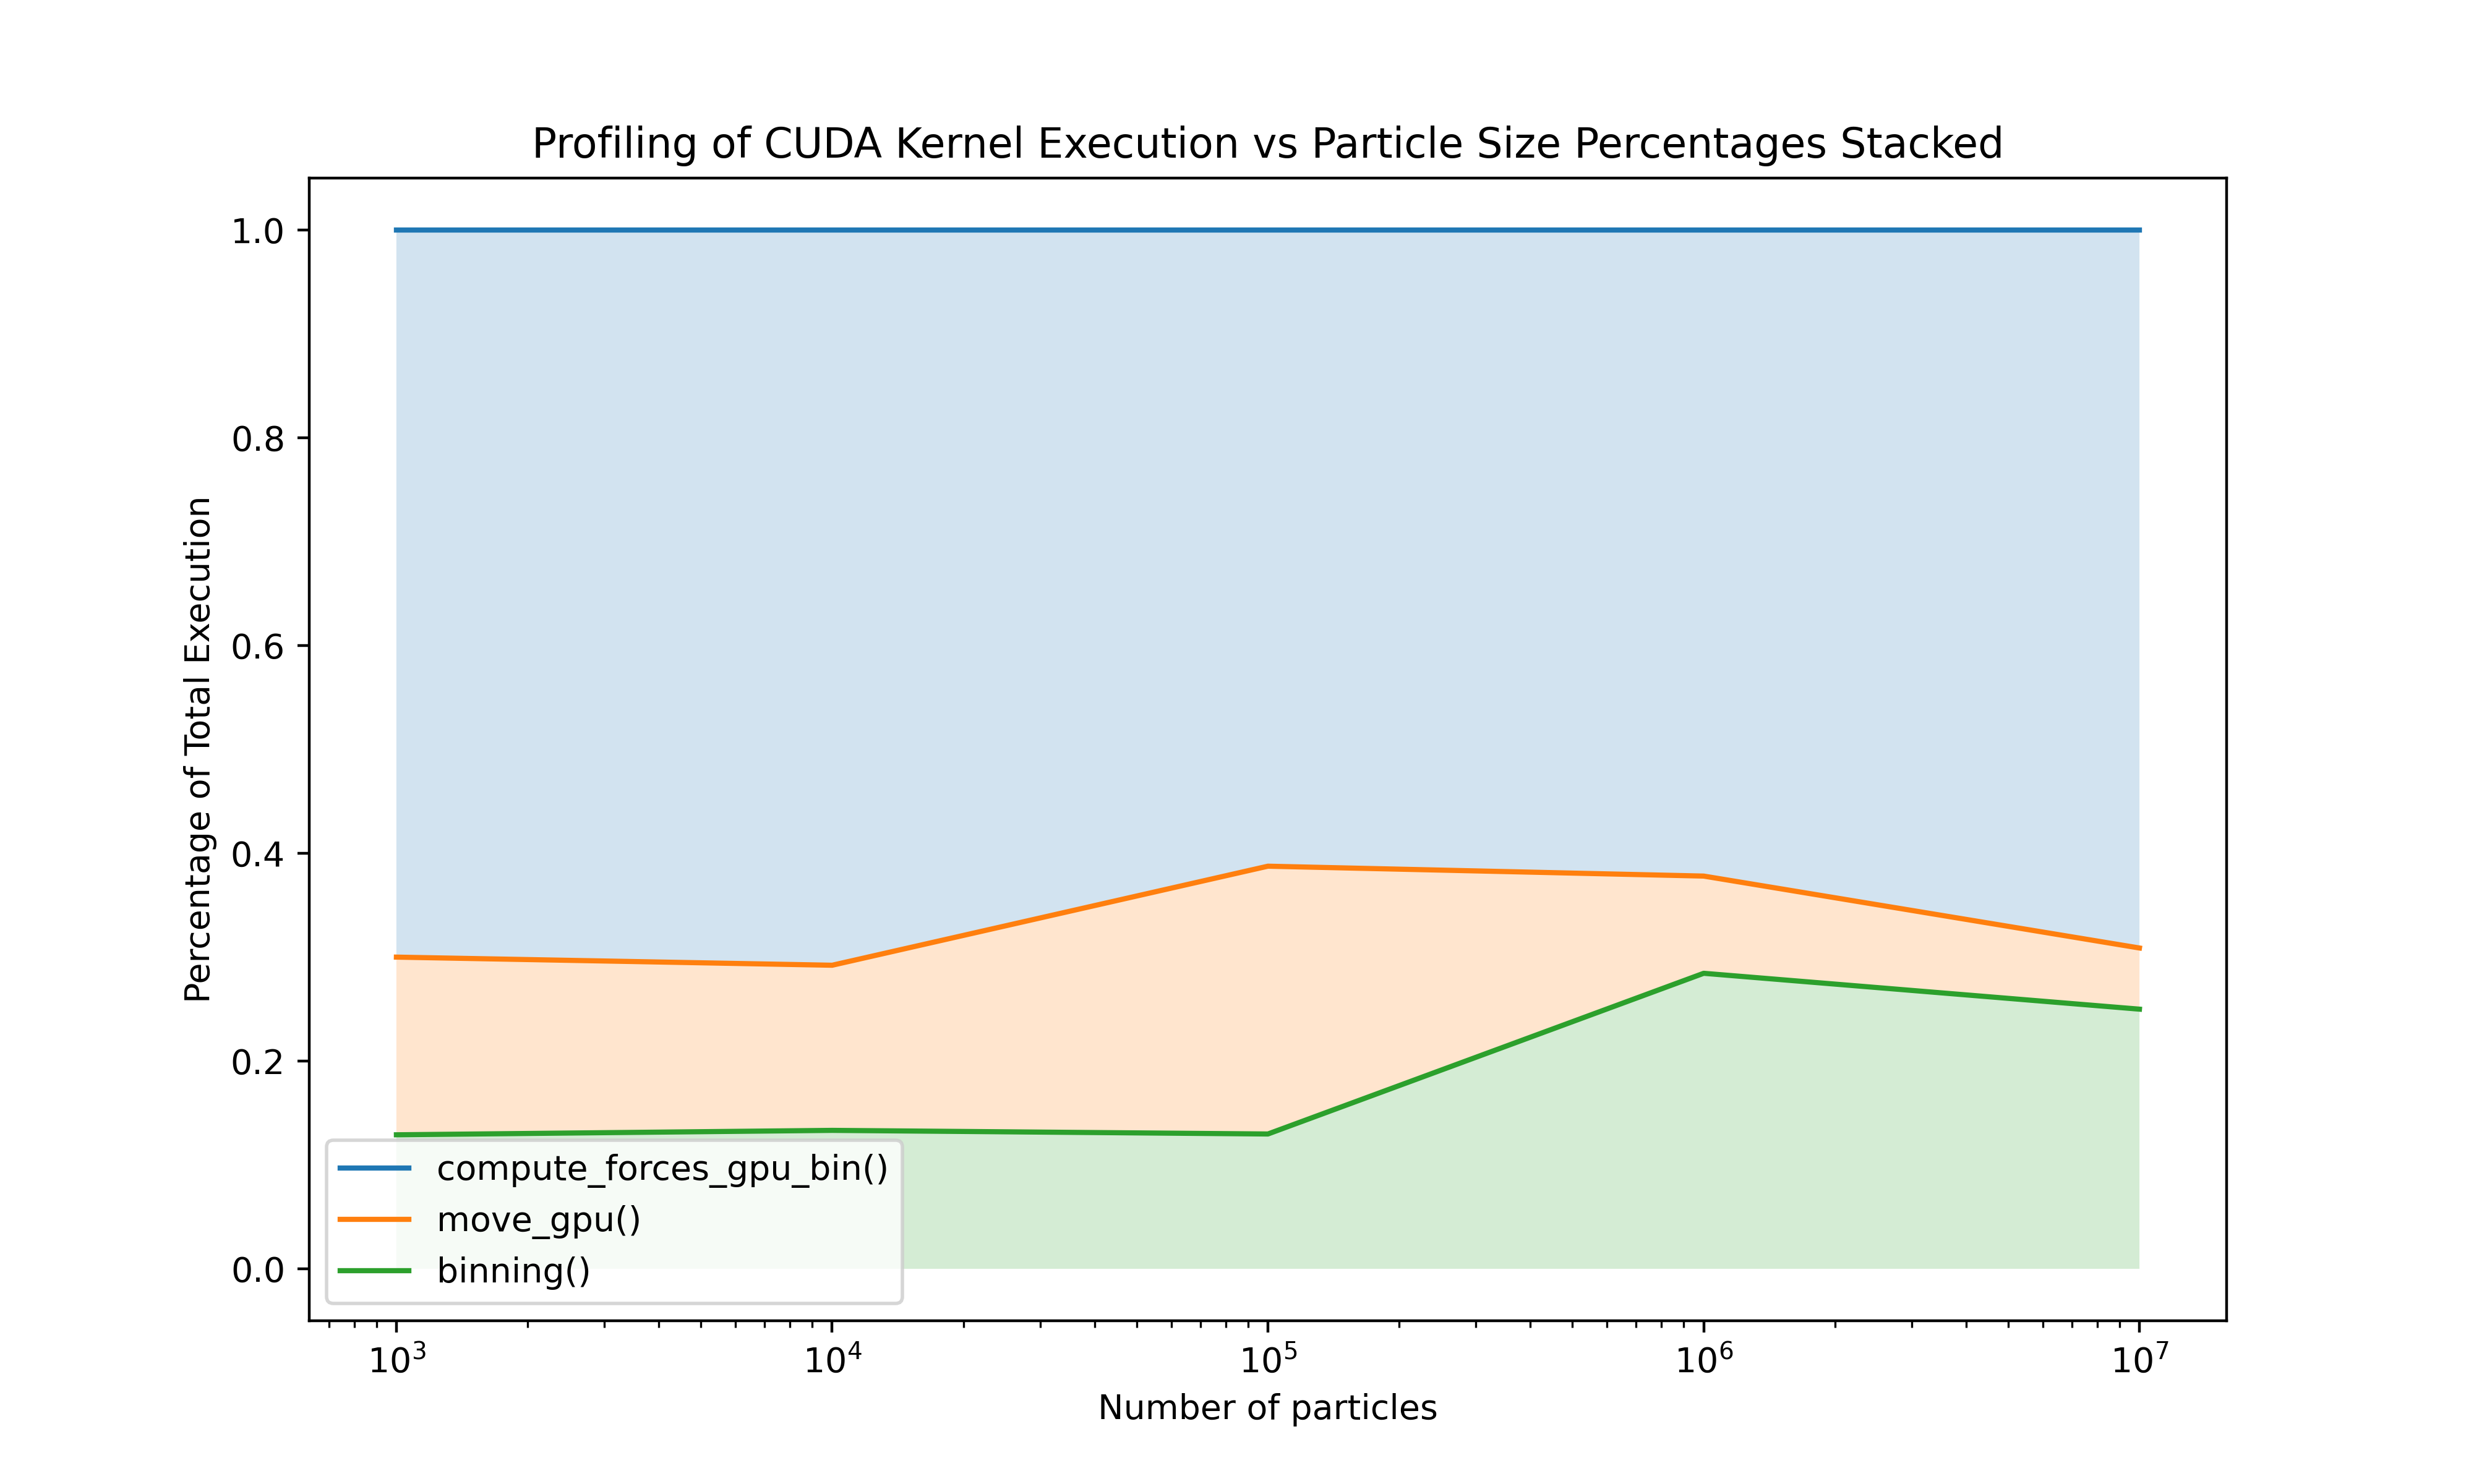
\includegraphics[width=6in]{figures/profiling-stacked-percentage.png}}


\section{Contribution}
Brian contributed to all of the code and report. The record breaking 1.26s simulation for 1 million particles was done by him. Andrew helped with a few edge cases and debugging. Xuan explored some other solutions.

\end{document}

